

%! TeX program = lualatex

{}\documentclass[a4paper]{article}
% {}\documentclass[a4paper,landscape]{article}
% {}\documentclass[a4paper,landscape,twoside]{article}

%-----------------------------------------------------------------
% GENERAL PACKAGES
%-----------------------------------------------------------------
\RequirePackage[ddmmyyyy]{datetime} % change date format
\renewcommand{\dateseparator}{.} % select date separator character
\RequirePackage[shortlabels]{enumitem} % pause/resume lists
\RequirePackage{multicol} % multi column format
\RequirePackage{graphicx} % used for figures
\RequirePackage[dvipsnames]{xcolor} %colors, dvips -> extra premade colors
\RequirePackage[explicit]{titlesec} % formating of titles
\RequirePackage{siunitx} % SI units
\usepackage{amsmath, amssymb} % For mathematical symbols and equations
\RequirePackage{mathtools} % even more math stuff
\RequirePackage{subcaption}
\RequirePackage[hidelinks]{hyperref} % used for hyperlinked nodes
\RequirePackage[document]{ragged2e} % left ragged text
\RequirePackage{atbegshi}  % special commands that apply tikz to all pages
\RequirePackage{etoolbox} % Boolean and if/else
\RequirePackage{calc} % math inside other commands
\RequirePackage{booktabs}
\RequirePackage{lipsum}
\usepackage{float} % For [H] specifier
\usepackage{parskip} % For paragraph spacing
\usepackage{longtable}
\usepackage{tcolorbox}
%-----------------------------------------------------------------
% FONT
%-----------------------------------------------------------------
\usepackage{fontspec}
\usepackage[ngerman]{babel}
% \babelfont{rm}{Lato}
% \babelfont{rm}{Roboto}
\babelfont{rm}{Roboto Condensed}
% \babelprovide[onchar=ids fonts]{russian}
% \babelfont[russian]{rm}{Roboto Condensed}
\babelprovide{english}
% font of math
% \usepackage{lmodern} # default
% \usepackage{newtxmath}
% \usepackage{mathpazo}
% Custom command for transpose with thinner T
\newcommand{\trans}{\textnormal{\scriptsize T}}
%-----------------------------------------------------------------
% TOGGLE
%-----------------------------------------------------------------

\newtoggle{do-multicol}
\togglefalse{do-multicol}
%-----------------------------------------------------------------
% \newtoggle{showLecture}
% \toggletrue{showLecture}
% \togglefalse{showLecture}
% \newtoggle{showRecital}
% \toggletrue{showRecital}
% \togglefalse{showRecital}
%-----------------------------------------------------------------
% GEOMETRY
%-----------------------------------------------------------------
%%% regular a4 layout, f.e. 2col
%-----------------------------------------------------------------
% \RequirePackage[
% 	paperheight=297mm,
% 	paperwidth=210mm,
% 	top=19mm,
% 	bottom=19mm,
% 	footskip=5mm,%TODO
% 	inner=19mm,
% 	outer=19mm,
% 	centering
% ]{geometry}
%-----------------------------------------------------------------
% column settings (% comment for regular  column)
% \toggletrue{do-multicol}
% \def\numcolumns{2} 
% \setlength{\columnsep}{19mm}
%-----------------------------------------------------------------
% % %%% tight a4 landscape layout
%-----------------------------------------------------------------
% % paper settings
% \RequirePackage[
% 	paperheight=210mm,
% 	paperwidth=297mm,
% 	top=1mm,
% 	bottom=1mm,
% 	inner=1mm,
% 	outer=1mm,
% 	centering
% ]{geometry}
% % column settings
% \toggletrue{do-multicol}
% \def\numcolumns{4} 
% \setlength{\columnsep}{3mm}
% % set pagestyle (remove pagenumbering)
% \pagestyle{empty}
%-----------------------------------------------------------------
% \usepackage[skip=0.2mm]{caption} % Reduces space between image and caption
% \captionsetup{font={footnotesize,sf}}
% %-----------------------------------------------------------------
% \setlength{\intextsep}{0.2mm} % Space above/below in text
% \setlength{\textfloatsep}{0.2mm} % Space between floats
% \setlength{\floatsep}{0.2mm} % Space between floats
% % -----------------------------------------------------------------
% % space around title and fontsize
% \makeatletter
% \renewcommand{\section}{\@startsection{section}{1}{\z@}%
% 	{.5mm}% % Space before
% 	{.5mm}% % Space after
% 	{\normalfont\normalsize\bfseries}}
% 	% {\normalfont\normalsize\bfseries\color{RoyalBlue}}}
% \renewcommand{\subsection}{\@startsection{subsection}{2}{\z@}%
% 	{.25mm}%
% 	{.25mm}%
% 	{\normalfont\small\bfseries}}
% 	% {\normalfont\small\bfseries\color{RoyalBlue}}} % Add color to subsection
% \makeatother
% %-----------------------------------------------------------------
% \renewenvironment{quote}
% {\list{}{\rightmargin0mm\leftmargin0mm}
% 	\item\relax\centering\arraybackslash}
% % {\endlist\vspace{0mm}} 
% {\endlist\vspace{-1mm}}
% %-----------------------------------------------------------------
% % %% indent for paragraph
% \setlength{\parindent}{0mm}
% % %% space between paragraphs
% \setlength{\parskip}{0mm}
% % %% spacing within lists
% \setlist{itemsep=0mm, topsep=0mm} % For all itemize/enumerate
% \setlist[itemize]{itemsep=0pt, leftmargin=3mm}
% \setlist[enumerate]{itemsep=0pt, leftmargin=4mm}
%-----------------------------------------------------------------
% %%% very small for 1 col preview
%-----------------------------------------------------------------
\RequirePackage[
	paperheight=297mm,
	paperwidth=95mm,
	top=1mm,
	bottom=1mm,
	inner=1mm,
	outer=1mm,
	centering
]{geometry}
% -----------------------------------------------------------------
% THEOREM STYLE
%-----------------------------------------------------------------
\usepackage{amsthm} % For definition environment
% Define the definition environment
\theoremstyle{definition}
\newtheorem{definition}{Definition}
% Define the theorem environment
\theoremstyle{definition}
\newtheorem{theorem}{Theorem}
% Define the proposition environment
\theoremstyle{definition}
\newtheorem{proposition}{Proposition}
%-----------------------------------------------------------------
% OTHER FORMATTING
%-----------------------------------------------------------------
% \pagestyle{empty}
% \pagestyle{plain}
% -----------------------------------------------------------------
% create lines between columns and define color of columns
% \setlength{\columnseprule}{.3mm} %set thickness default 1pt
% \def\columnseprulecolor{\color{RoyalBlue!20}}
% -----------------------------------------------------------------
\usepackage{sectsty}
\setcounter{secnumdepth}{1} % Number subsections (##)

% -----------------------------------------------------------------
% INHALT
%-----------------------------------------------------------------

\begin{document}

\iftoggle{do-multicol}{
	\begin{multicols}{\numcolumns}}{}
		%-----------------------------------------------------------------
		
%-----------------------------------------------------------------
% two boxes centered with date below
%-----------------------------------------------------------------
\begin{center}
	\colorbox{RoyalBlue}{\textcolor{white}
		{\makebox[\linewidth][c]{
				\Large{\textbf{
						Large-Scale Convex Optimization
					}}}}}
	\colorbox{lightgray}{\textcolor{Black}
		% \colorbox{BrickRed}{\textcolor{White}
		{\makebox[\linewidth][c]{
				\normalsize{
					\textbf{Silvan Stadelmann}
					% Silvan Stadelmann}
					\url{silvasta@ethz.ch}
				}\scriptsize{
					\selectlanguage{german}{\today{}}
					% \today{}
				}}}}
\end{center}




% \normalsize{
% 	% \textbf{Stadelmann Silvan}}
% 	Stadelmann Silvan}
% \small{
% 	\url{silvasta@ethz.ch}
% 	\selectlanguage{german}{\today{}}
% 	% \today{}
% }}}}

		% footnotesize
		%-----------------------------------------------------------------
		% sections
		% \section{Introduction}

\textbf{Large Scale}
Problem of dimension $n$ but iterations $\ll n$ desired

\textbf{Convex}
One of the only problem classes that are \textquote{solvable}

\textbf{Mathematical Optimization}
\begin{equation}
	\begin{aligned}
		\operatorname{minimize} & f(x)                               \\
		\text{s.t.}             & g_i(x) \le 0,\quad i = 1,\dots,n_g \\
		                        & h_i(x) = 0,\quad i = 1,\dots,n_h   \\
	\end{aligned}
	\label{eq:optimization}
\end{equation}

- $x = (x_1,...,x_n) \in \mathbb{R}^{n}$ decision variable

\quad (most of our algorithms also work for $n\rightarrow\infty$)

- $f$ objectivce function

- $\mathcal{C} = \{\xi \in \mathbb{R}^{n}: g(\xi)\le0,\ h(\xi)=0\}$ fesabile set

\subsection{Important Definitions}

- $x^\star$ is a \textit{global minimum} if $f(x^*)\leq f(x)$

- $x^\star$ is a \textit{local minimum} if there exists $\epsilon > 0$ s.t.
$$f(x^\star)\leq f(x) \quad \forall x \in C \cap B_\epsilon(x^\star)$$
$B_\epsilon(x^\star):=\{\xi\in\mathbb{R}^{n}:|\xi-x^\star|<\epsilon\}$ open ball, center $x^\star$, radius $\epsilon$

\subsection{Existance of minimum}

\subsubsection{Counter examples}

a) unbounded level sets, f.e. $1/x$

b) $C$ open f.e. $(0,1)$ but minimum at f.e. $0$

c) $f$ not l.s.c. (lower semi-continuous)

% todo Grafik
%
\begin{proposition}
	$f$ (lower-semi-)continuous,
	$f(x)\rightarrow\infty$ for $|x|\rightarrow\infty$,
	$\mathcal{C}$ closed
	$\Rightarrow$ \exists\ minimizer of (\ref{eq:optimization}) described by:
	$
		\min_{x \in \mathcal{C}} f(x) \text{\ and\ } \underset{x \in \mathcal{C}}{\operatorname{argmin}} f(x) % todo check argmin
	$
\end{proposition}


\subsubsection{Examples}

% todo find best way for items
$x$:

- assets in a portfolio

- control inputs

- schedule assignment

- resource allocation

$\mathcal{C}:$

- all possible trade assets

- actuation limits

$f$:

- cost (negative returns)

- deviaton from target

- waiting times / delas

- risk (a certain resource fails)

\subsubsection{First Order Algorithmus}

% todo pseudo algorithm
Initialize $x_0$

for k = 0,...,\#iterations -1

$(f(x_k),\nabla f(x_k))$ <-- call first-order oracle

Determine $x_{k+1}$ based on ${..f..}$

end

Analythic, arithmetic complexity

\begin{definition}[Lipschitz continuity]
	$q: \mathbb{R}^{n} \rightarrow \mathbb{R}^{m}$
	is Lipschitz with constant $L$ if:
	$|q(x)-q(y)| \le L |x-y| \forall x,y \in \mathbb{R}^{m}$
\end{definition}

Class of OP $P$ with $\mathcal{C}=[0,1]^n$
and $f$ is $l^\infty$-Lipschitz

\begin{proposition}
	For any algorithm $\exists$ problem in $P$,
	s.t. achieving $|f(x_N )−f(x^⋆)| < \epsilon$
	requires
	$$N \ge \left(\left\lfloor\frac{L}{2\epsilon}\right\rfloor\right)^n-1$$
	%TODO: check frac
\end{proposition}

\textbf{Example}

(for L=1, $\epsilon$ = 0.0005, n=27, N larger than \#atoms in universe)

\begin{proof}[Proof]
	\textbf{Idea}
	Construct $f$ where $(f(x_0) = 0,\nabla f(x_0) = 0)$, $(f(x_1) = 0,\nabla f(x_1) = 0),...$ but the actual $min_{x \in C}f(x)$ is small.

	\textbf{Grid(x1,x2)}

	raster 1/3, 9 boxes in (1,1), for $N\le 7$ (8 steps) one grid cell is not visited

	Hence $f(x_i) = 0, i \in [0,7]$ but $f(x^*) = -L/6$

	\textbf{Generalization}

	- Partition unit cube into $s^n$ small boxes with side length $1/s$ and $min_xinC = -L/2s$
	- therefore $f(x_i)-f(x_star) \ge L/2s$ for $i=0...s^n-2$
	- roughly ...
	- therefore $N=$ ...
	%TODO: Proof

\end{proof}

\begin{definition}[]
	The optimization problem \ref{eq:optimization} is convex
	if $f$ and $g_i$ are convex functions,
	$i = 1, . . . , n_g$ ,
	and $h$ is affine.
\end{definition}

\begin{definition}[]
	Function $q: \mathbb{R}^{n}\rightarrow\mathbb{R}$
	is convex (affine)
	if for any $x, y \in \mathbb{R}^{n}$
	$$
		q(\theta x+(1 − \theta)y) \le \theta q(x) + (1 − \theta)q(y)\quad\forall\ \theta \in [0, 1]
	$$
\end{definition}

\subsubsection{Software Frameworks}

- CVX Python
- Yalmip

\begin{proposition}
	$x^\star$ local minimum of (\ref{eq:optimization}),
	if (\ref{eq:optimization}) convex,
	then $x^\star$ global minimum of (\ref{eq:optimization})
\end{proposition}


\begin{proof}[Proof ]
	Counter example, $\exists$ $y\ne x^\star \in C$ such that $f(y)\le f(x^\star)$
	%TODO: Proof
\end{proof}

%TODO: Ackley Function

		% \section{Convex sets and convex functions}

\begin{definition}[Convex Set]
	A set $\mathcal{C}$ is convex if and only if
	$\forall x,y \in \mathcal{C}$ and
	$\forall \theta \in [0,1]$: \quad
	$\theta x + (1-\theta)y \in \mathcal{C}$.
\end{definition}


\textbf{Examples of convex sets:}
\begin{itemize}
	\item
	      hyperplane $\{x \in \mathbb{R}^n \mid a\T x=b\}$
	\item
	      half-space $\{x \in \mathbb{R}^n \mid a\T x\le b\}$
	\item
	      polyhedron $\{x \in \mathbb{R}^n \mid Ax \preceq b ,\ Cx = d\}$

	      $A \in \mathbb{R}^{q\times n},\ C \in \mathbb{R}^{r\times n},\ b \in \mathbb{R}^{q},\ d\in \mathbb{R}^{r}$
	\item
	      ...more...

\end{itemize}

\subsection{Operations that preserve convexity (sets)}

\begin{itemize}
	\item \textbf{Intersection}
	      $\mathcal{C}_1, \mathcal{C}_2$ convex $\Rightarrow \mathcal{C}_1 \cap \mathcal{C}_2$ convex
	\item \textbf{Image under affine map}
	      $\mathcal{C} \subseteq  \mathbb{R}^{n}$ convex
	      $\Rightarrow \{Ax+b \mid x \in \mathcal{C} \}$ convex
	\item inverse image of an affine map:
	      ...
\end{itemize}

\subsection{Separating Hyperplane Theorem}

\begin{theorem}
	$\mathcal{C} \subseteq \mathbb{R}^{n}$ non-empty closed convex set, $y \notin \mathcal{C}$
	$\rightarrow \exists\ a \ne 0, b \in \mathbb{R}$
	s. t. $a\T x + b < a\T y + b,
		\forall x \in \mathcal{C}$
\end{theorem}

\begin{proof}
	\textbf{Claim}
	$\exists\ \hat{x} \in C$ s.t. $|\hat{x}-y|\leq |x-y|\quad \forall x \in \mathcal{C}$

	\textbf{Proof of claim}
	$|x-y|$ has bounded level sets,
	$\mathcal{C}$ is non-empty and closed
	$\Rightarrow \exists\ \hat{x} \in \underset{x \in \mathcal{C}}{\operatorname{argmin}}|x-y|$

	Hyperplane, we choose $a:=y-\hat{x}, b:=-a\T\hat{x} = -(y-\hat{x})\T\hat{x}$

	As a result, $a\T x + b = (y-\hat{x})\T (x-\hat{x})$
	and therefore $a\T y + b = |y-\hat{x})|^2 > 0$.
	The following claim shows that the hyperplane $a\T y + b$ seperates $\mathcal{C}$ and $y$.


	\textbf{Claim}
	$a\T y + b \le 0\quad \forall x \in \mathcal{C}$

	\textbf{Proof of claim}
	Assume not.
	$\rightarrow \exists\ x \in \mathcal{C}$ s.t.
	$(y-\hat{x})\T (x-\hat{x}) > 0$

	PARAMETRIZE $\theta$

	Contradiction $\hat{x}$ nearest point to $y$

	(Details in Lecture notes)
\end{proof}

\begin{corollary}
	A closed convex set $\mathcal{C} = \mathbb{R}^n$
	is the intersection of the closed half-spaces
	that contain $\mathcal{C}$.
\end{corollary}

\begin{proof}
	$\mathcal{S}$ intersection of closed half-spaces that contain $\mathcal{C}$

	1) $\mathcal{C} \subseteq \mathcal{S}: x \in \mathcal{C}$
	$\Rightarrow x$ is contained in every half-spaces that contains $\mathcal{C}$
	$\Rightarrow x$ is also contained in the intersections of half-spaces that contains $\mathcal{C}$
	$\Rightarrow x \in \mathcal{S}$

	2) $\mathcal{S} \subseteq \mathcal{C}:$
	Assume not
	$\rightarrow\ \exists\ \hat{x}\in \mathcal{S}$
	with $\hat{x}\notin \mathcal{C}$.
	By the Seperating Hyperplane Theorem there exists a hyperplane
	that seperates $\hat{x}$ from $\mathcal{C}$.
	That means there exists a closed half-space
	that contains $\mathcal{C}$ but not $\hat{x}$,
	hence $\hat{x}\notin \mathcal{C}$, contradiction.
\end{proof}

\subsection{Support function}

\textbf{Idea} represent any closed convex set by its supporting hyperplanes

Support Function: $\sigma_\mathcal{C}(a) = \underset{x \in \mathcal{C}}{\operatorname{sup}}a^Tx$

CALCULATION EXAMPLE

If we know the $\sigma_\mathcal{C}(a)$, we arrive at at

$$  \mathcal{C} = \bigcap_{a \in \mathbb{R}^n} \{x \in \mathbb{R}^n \mid a\T x - \sigma_c(a) \leq 0\}$$

$$   = \{x \in \mathbb{R}^n \mid \underset{a \in \mathbb{R}^{n}}{\operatorname{sup}}\ a\T x - \sigma_\mathcal{C}(a) \le 0\}$$

\begin{definition}
	A function $f : \mathbb{R}^n \rightarrow \mathbb{R}$
	is convex if and only if its epigraph is a convex set, where
	$$\operatorname{epi}(f):=\{(x,t)\in \mathbb{R}^{n+1} | f(x) \le t \}$$
\end{definition}

$\rightarrow$ this provides a link between convex sets and functions

\subsection{Operations that preserve convexity (functions)}

\begin{itemize}
	\item the pointwise maximum of convex functions is convex
	\item the sum of convex functions is convex
	\item $f(Ax+b)$ is convex if $f$ is convex
\end{itemize}

\subsubsection{How to check if f is convex?}

\begin{itemize}
	\item if $f: \mathbb{R}^n \rightarrow \mathbb{R}$ twice differentiable,
	      $\partial^2f/\partial x^2 \succeq 0\ \forall\ x \in \mathbb{R}^{n}$

	\item if $g: \mathbb{R} \rightarrow \mathbb{R}$ with $g(t)=f(x+tv)$
	      convex in $t\ \forall\ x,v \in \mathbb{R}^{n}$,
	      then $f$ is convex
	\item composition of simple convex function with convexity preserving operations
\end{itemize}

\textbf{Extended real numbers} $\bar{\mathbb{R}} = \mathbb{R} \cup \{+\infty, -\infty\}$


\textbf{Indicator function}
$\psi_\mathcal{C}(x) := \begin{cases} +\infty &\text{if } x \notin\mathcal{C} \ge 0 \\ 0 &\text{if } x \in\mathcal{C} \end{cases}$

$\rightarrow$ this provides another link between convex sets and functions

We can write
$\min_{x \in \mathcal{C}}f(x)$ as
$\min_{x \in \mathbb{R}^{n}}f(x) + \psi_\mathcal{C}(x)$

\begin{definition}[3]
	$f: \mathbb{R}^{n}\rightarrow\bar{\mathbb{R}}$ is called proper
	if $f$ is bounded below and
	if $\exists\ x \in \mathbb{R}^{n}$ s. t. $f(x)<\infty$
\end{definition}

\begin{definition}[Legendre Transformation]
	The conjugate function of $f: \mathbb{R}^{n}\rightarrow\bar{\mathbb{R}}$  is defined as
	$f^\star(y)=\underset{x \in \mathbb{R}^{n}}{\operatorname{sup}}y\T x-f(x)$
\end{definition}

IMAGE F-STAR

\subsection{Summary of Concepts}

% \begin{figure}[H]
% 	\centering
% 	% \includegraphics[width=\columnwidth]{images/X}
% 	\caption{cap}
% \end{figure}

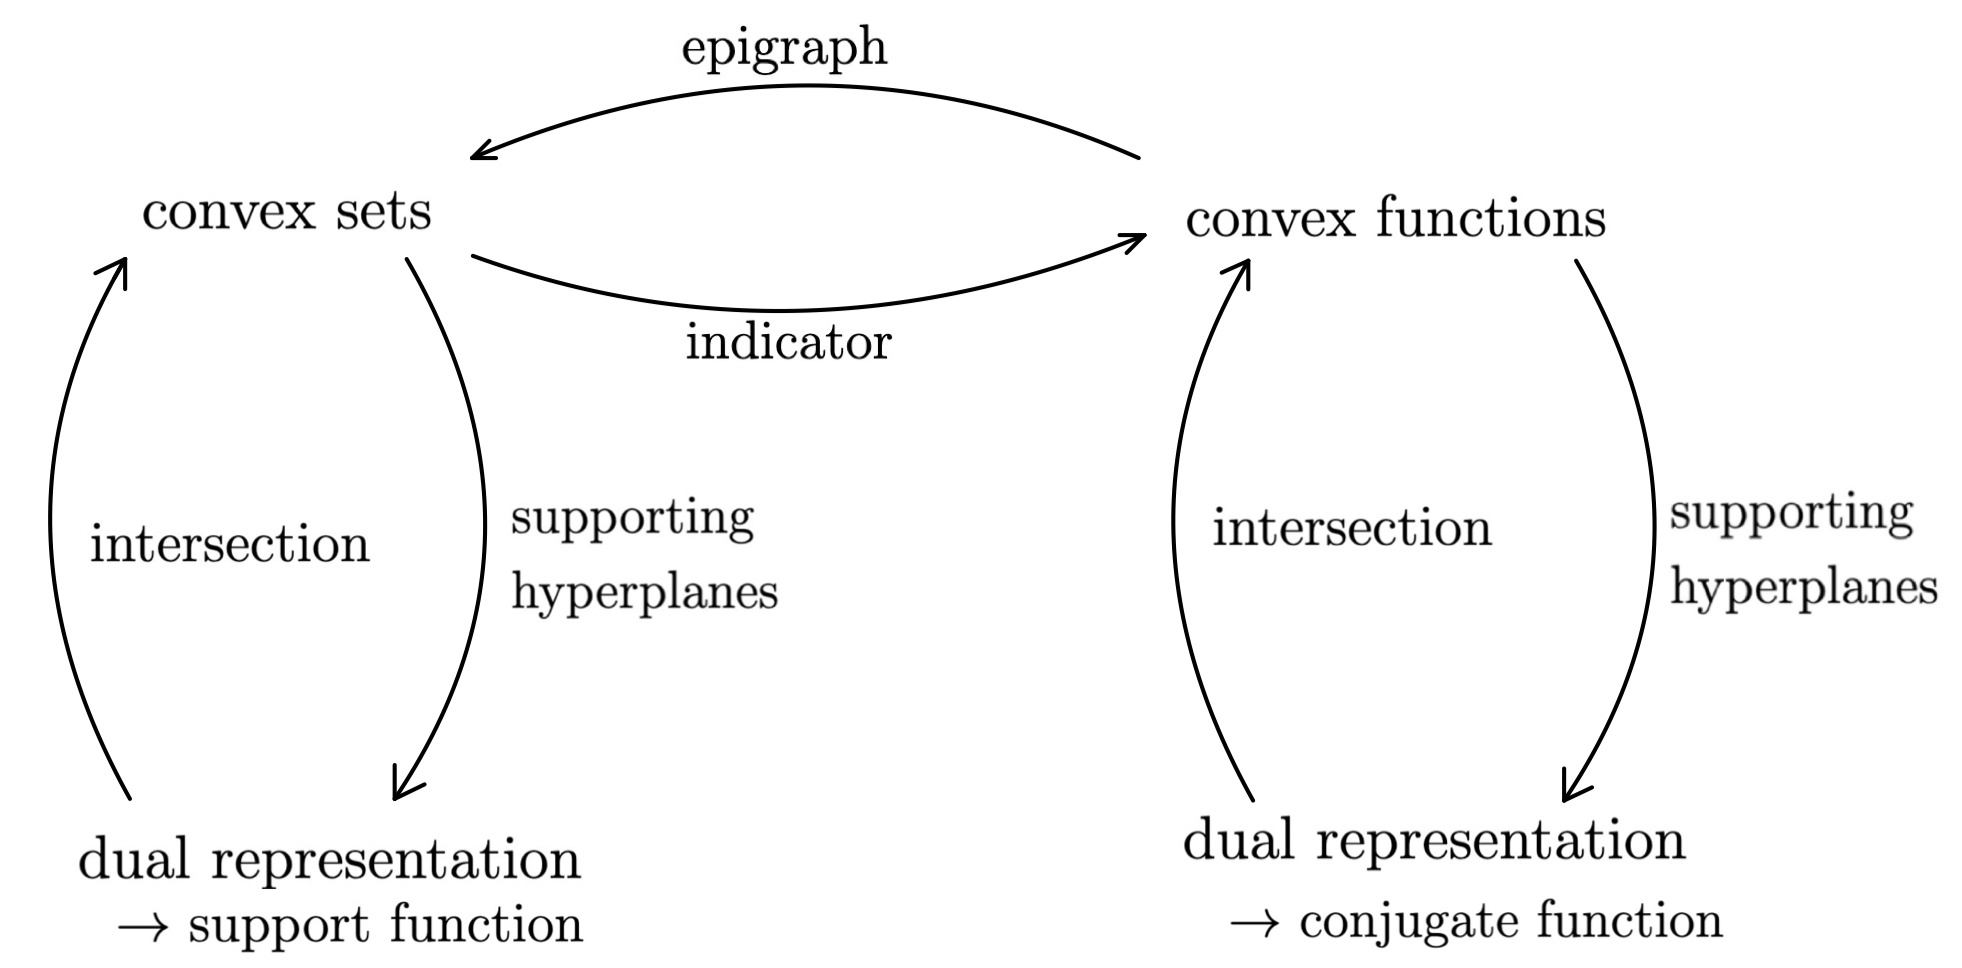
\includegraphics[width=\columnwidth]{images/summary_set_functions.png}

QUESTION

Theorem 2

		\subsection{Recitation}

\subsubsection{Convex Sets}

A set $\mathcal{C}$ is convex if and only if for all
$x,y \in \mathcal{C}$ and $\theta \in [0,1]$:
$$\theta x + (1-\theta)y \in \mathcal{C}$$

\subsubsection{Convex Cone}

conic combination

Given $x_1,...,x_n$

any point of the form:

$\theta_1 x_1,...,\theta_n x_n$

$\theta_i \ge 0$

convex cone

XXX

\subsubsection{Positive Semidefinite Cone}

Notation

$\mathbb{S}^n$ set of symetric nxn matrices

$\mathbb{S}_+^n$ HHH

$\mathbb{S}_{++}^n$ HHH not convex cone

Example

Sylvester Condition

\subsubsection{Convex Functions}

Definition

\subsubsection{Methods for establishing convexity}

1. Verify from definition

2. Second order condition

3. Operations that preserve convexity

\subsubsection{Log-Sum-Exp}

$$f(x) = log(e^x_1+...+e^x_n)$$

differentiable approximation of max(x)

How to check convexity?

Second-order condition $\nabla^2f\ge 0$

\subsubsection{Nonnegative Weighted Sum}

$\alpha(f_1 + f_2)$ convex if $f_1, f_2$ convex, $\alpha > 0$

$f_1,\dots,f_m$ convex, $w_1,\dots,w_m \ge 0$
$\Rightarrow w_1f_1+\dots+w_mf_m$ convex

\subsubsection{Composition with Affine Function }

$$g(x) =f(Ax+b) $$

Examples

Log barrier for linear inequalities
$\rightarrow$ transforms constrained problem in unconstrained

Norm Function

\subsubsection{Composition}

$$f(x)=h(g(x))$$

		\section{KKT and Lagrange Duality}

\subsection{Example}

Optimization problem:
$\min _{x \in \mathbb{R}^2} f(x)$ s.t. $h(x)=0$

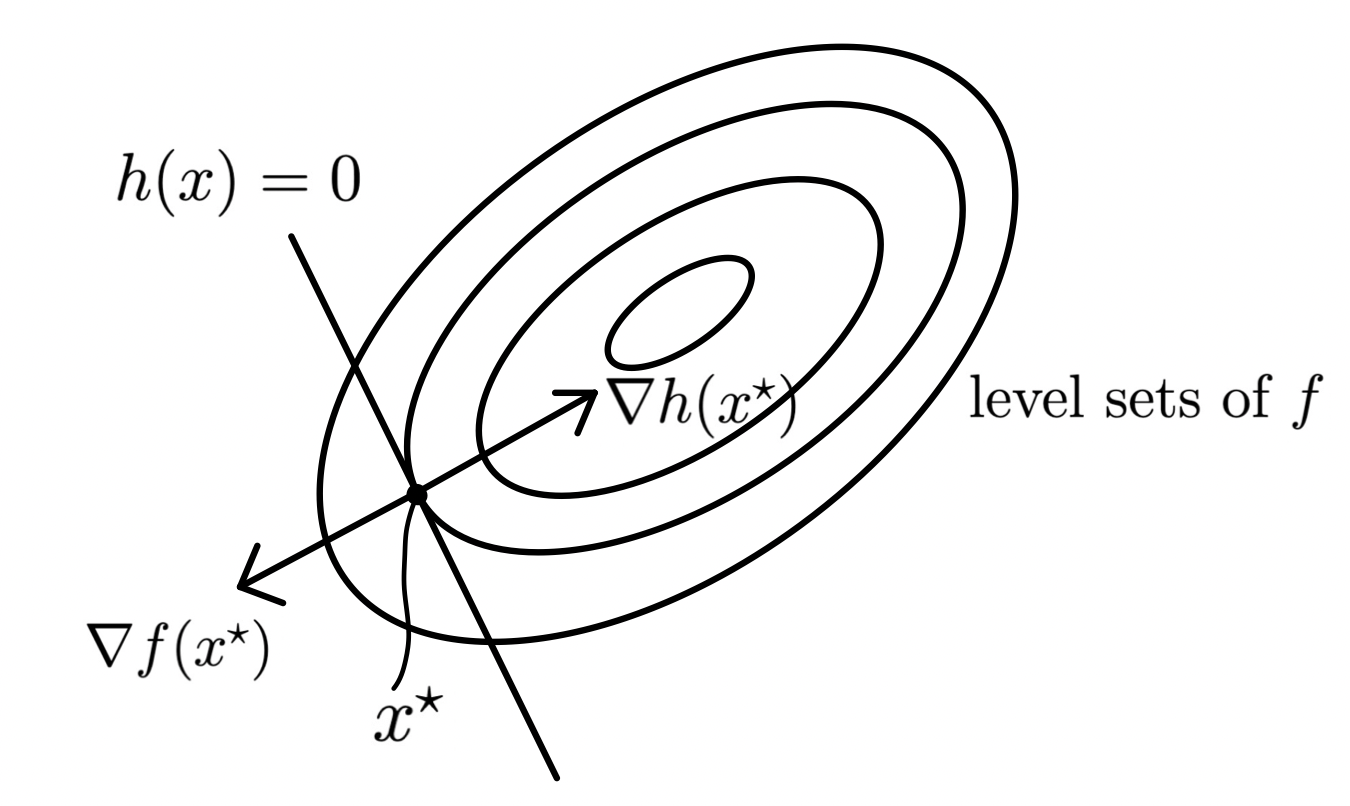
\includegraphics[width=\columnwidth]{images/op_eq_constraints.png}

We note the following:
$\nabla f(x^\star)$ and $\nabla h(x^\star)$ are colinear


$\Leftrightarrow \exists\ \nu^\star \in \mathbb{R}: \nabla f(x^\star)+\nu^\star\nabla h(x^\star) = 0$

$f(x)+\nu^\star h(x)$ is stationary at $x^\star$,
where $\nu^\star$ can be interpreted as cost of violationg constraint

\subsection{Generalization}

Generalization to $n \ge 2$ and presence of inequality constraints

\begin{equation}
	f^\star = \underset{x \in \mathcal{\mathbb{R}}^n}{inf}f(x) \text{ s.t. } h(x)=0,\ g(x) \le 0
	\label{eq:dual}
\end{equation}

with corresponding Lagrange function
\begin{equation}
	\mathcal{L}(x,\lambda,\nu) = f(x) + \lambda\T g(x)+\nu\T h(x)
\end{equation}

where $\lambda_i \ge 0, \nu_i \in \mathbb{R}$ are the dual variables or multipliers
that can be interpreted as cost for violationg constraints.

\begin{proposition}[Weak Duality]
	The  dual function

	$d(\lambda,\nu) = \underset{x \in \mathcal{\mathbb{R}}^n}{inf}\mathcal{L}(x,\lambda,\nu)$ satisfies

	$d(\lambda,\nu)\le f^\star,\ \forall \lambda\ge 0,\ \nu \in \mathbb{R}^{n_h}$

\end{proposition}

\begin{proof}
	SHORT %TODO  
\end{proof}

\begin{definition}[Constraint  qualification]
	$\mathcal{C}$ convex, Slaters Condition holds if
	$\exists\ \hat{x} \in \mathbb{R}^{n}$ s.t. $h(\hat{x})=0$ and $g(\hat{x})<0$
\end{definition}

\begin{proposition}[Strong Duality]
	If Slater's condition holds and (\ref{eq:dual}) is convex then
	$\exists \lambda \ge 0, \nu \in \mathbb{R}^{n_h}$ s.t. $d(\lambda,\nu)=f^\star$
\end{proposition}

\begin{proof}
	EXTENDED %TODO
	GRAPHIC
\end{proof}

\subsection{KKT}

\begin{theorem}[KKT Conditions]
	Slater's condition holds and (\ref{eq:dual}) is convex.
	Then $x^\star \in \mathbb{R}^{n}$ is a minimizer of the primal (\ref{eq:dual})
	and $(\lambda^\star \ge 0,\ \nu^\star) \in \mathbb{R}^{n_g} \times \mathbb{R}^{n_h}$ is a maximizer of the dual
	if and only if: %todo align
	$$ KKT-1\ (Stationary\ Lagrangian)                                         $$
	$$ \nabla_x\mathcal{L}(x^\star,\lambda^\star,\nu^\star)=0                 $$
	$$ KKT-2\ (primal\ feasibility)                                           $$
	$$ g(x^\star)\le0, h(x^\star)=0                                           $$
	$$ \quad\ KKT-3\ (dual\ feasibility)                                      $$
	$$ \lambda^\star\le0, \nu^\star \in \mathbb{R}^{n_h}                      $$
	$$ \quad\ KKT-4\ (complementary\ slackness)                               $$
	$$ {\lambda^\star}\T g(x^\star)=0,\ {\nu^\star}\T h(x^\star)=0     $$

	In addition we have:
	$INF=SUP$ %todo

\end{theorem}

QUESTION Proof?

\textbf{Remark} Without Slater,
KKT 1 to 4 still implies $x^\star$ minimizes (\ref{eq:dual})
and (\lambda,\nu) maximizes the dual,
but the converse is no longer true,
there can be primal/dual minimizer maximizer that do not satisfy KKT1-4

FORCE BALLANCE %todo

\subsection{What if $f, g$ not differentiable?}

\textbf{Example} $\underset{x \in \mathcal{\mathbb{R}}^n}{inf}|Ax -b|^2 + |x|_1$

where $\mathcal(l_1)$-norm not  differentiable at 0

\subsection{Subdifferential}

for  convex  f... %todo

\begin{definition}
	$f: \mathbb{R}^{n} \rightarrow \bar{\mathbb{R}}$ convex,
	the subdifferential of $f$ at $\bar{x}$ is:
	$\partial f(\bar{x}):= \{\lambda \in \mathbb{R}^{n} \mid f... \}$ %todo
\end{definition}

\begin{proposition}[]
	$f: \mathbb{R}^{n} \rightarrow \mathbb{R}$ convex.
	$x^\star \in argmin...$
\end{proposition}

\begin{proposition}[Relation to conjugate functions]
	$f$ convex, $epi(f)$ closed:
	$y \in \partial f(x) \leftrightarrow x \in \delta f^\star(y)$
\end{proposition}



		\subsection {Recitation 3}

\subsubsection{Information ML}

\subsubsection{Hard Margin SVM}

Use hyperplane  and support vectors for data classification.

\subsubsection{SVM}
Find the Maximum-Margin Hyperplane

\subsubsection{Solve the Optimization Problem}
\begin{itemize}
	\item Introduce Lagrange multiplier $\alpha_i \ge 0$ for $i=1,2,\dots,N$

	      ...

	\item ...
	\item  Solve  $\alpha^\star$ by Strong Duality
	\item Obtain $w^{\star}$ and $b^{\star}$ using KKT

\end{itemize}

\subsubsection{Soft Margin SVM}
\begin{itemize}
	\item Introduce some \textit{slackness} $\xi$
	\item Point 2
\end{itemize}

\subsubsection{Kernel Methods: Break the linearity}
Introduce  Nonlinear feature map $\phi(x): \mathbb{R}^{n}\rightarrow \mathbb{R}^{m}$

Kernel $K(x_i,x_j): \mathbb{R}^{n} \times \mathbb{R}^{m}\rightarrow \mathbb{R}$



		\section{Convex Optimization Problem}

minimize $f(x),g\le0,h(x)=0$

1) Feasibility  Problem

minimmize s

s.t. $g_i(x)\le s\quad \forall i,\dots,n_g$, $h(x)=0$

2) Linear Programming

minimmize $c^{\trans}x$ s.t. $Ax-b\ge0$ and $x\ge0$

$\rightarrow$ derive dual:

Step 1: $\mathcal{L}(x,\lambda_1,\lambda_1) = c^{\trans}x-\lambda_1^{\trans}(Ax-b) -\lambda_2^{\trans}x$

Step 2:$\underset{x \in \mathcal{\mathbb{R}}^n}{inf}\mathcal{L}(x,\lambda_1,\lambda_1)
	= \{-\infty else, \lambda_1^{\trans}b, if\ A^{\trans}\lambda_1+\lambda_2=c$

Step 3: Dual Problem

$\underset{\lambda_1 \ge0}{sup}\lambda_1 b$ s.t. $0\le c-A^{\trans}\lambda_2$

\begin{itemize}
	\item dual as a linear program
	\item Skech, polyhedron, c-vector normal gives 'Levelsets'
	      and optimal solution in or trough a corner (if exists)
\end{itemize}

\begin{proposition}
	The optimal solution of a linear program (if it exists)
	lies always on the boundary of the feasible set
	and there exists an optimal solution that is a vertex of the feasible set.
\end{proposition}

\textbf{Example} Shortest Path

Analogie with Fluid

Soltuion greater 0, not optimal edges = 0

3) Quadratic Programming

minimmize $\frac{1}{2}x^{\trans}Px+q^Tx$

s.t. $Gx\le h,\ Ax=b$

$\rightarrow$ if $P=P^{\trans}$ is positive semi-definite
then the problem is convex.


\textbf{Example} [optimal control] (basis for mpc)

% \subsubsection{Quadratically constrained quadratic program (QCQP)}

\subsubsection{Second-order cone program (SOCP)}

minimmize $f^Tx$

s.t. $|A_ix+b|\le c_i^Tx+d_i,\ Fx=g$

Cone: Cn+1=

\textbf{Example} [Markovitz portfolio optimization:]

\begin{itemize}
	\item $n$ number of assets/stocks
	\item $x_i$ relative value of asset $i$
	\item $p_i$ price change of stock $i$
	\item $p^Tx$ overall return
\end{itemize}

Constraints

\begin{itemize}
	\item $x^T\textbf{1} = B$, total amount
	\item $x\ge0$, no short position
\end{itemize}

CALCULATIONS

\subsection{Semidefinite programming (SDP)}

minimmize $c^{\trans}x$

s.t. $x_1F_1,\dots+x_nF_n <= 0$ and $Ax-b=b$

$\rightarrow$ the 'standard' form

$$\min _{x \in \mathbb{R}^{n*n}} tr(CX)$$


\textbf{Diagramm}

		\subsection{Recitation 4}

\subsubsection{Geometric Programming}

\textbf{Motivation}

- Summary Change of variables, transformation of objectives and constraints

\rightarrow convex problem in standard form

- Monomial function

- Posynomial function

- Problem formulation

- Example

- Technique

Variable transformation $y_i=\log{x_i}$ on objective and constraints.

- Transformation

\subsubsection{Sum of Squares}

- Polynomial Optimization

$\rightarrow f,g_i,h_i$ polynomials

General case intractable

- Nonnegative polynomials

Small adaption with \gamma

find largest \gamma such that $f(x)-\gamma$ nonnegative, NP Hard

$\rightarrow$ chose \gamma very high, results in sum of squares

\textbf{Definition}
A polynomial $f(x)$ is a sum of squares (SOS), if it can be written as
$$f(x) = \displaystyle\sum_{i}^{}g_i^2(x) \quad g_i \text{: polynomial}$$

- Verification

$z(x)$ as vector that contains all polynomials of degree $\le d$

\begin{theorem}[SOS]
	$p(x)$ is an SOS if and only if $\exists\ Q$ such that $Q >=0$ and $p(x)=z(x)\T Qz(x)$
\end{theorem}

Proof

Example

\textbf{SOS for Lyapunov Stability Analysis}

Dynamic

$\dot{x}_1 = -x_1^3+x_2$

$\dot{x}_2 = -x_1-x_2$

Equilibrium


$x = (x_1,x_2) = (0,0)$

$V(x) = ax1^2+bx2^2$
vdot = dVf(x)
= [2ax1,2bx2]*dynvec

verify vx>0,-vdot>0
%TODO

		\section{Gradient methods - Part I}

\begin{definition}[smoothness]
	The function $f : \mathbb{R}^{n}\rightarrow \mathbb{R}$ is $L$-smooth
	if $\nabla f(x)$ satisfies
	\[|\nabla f(x)-\nabla f(y)|\le L|x-y| \quad \forall x,y \in \mathbb{R}^{n}\]
\end{definition}

This result (with Taylors'Theorem) in:

\[f(y)\le f(x)+\nabla f(x)\T (y-x) +\frac{L}{2}|x-y|^2 \quad \forall x,y \in \mathbb{R}^{}\]

\begin{definition}[strong convexity]
	The function $f : \mathbb{R}^{n}\rightarrow \mathbb{R}$ is $\mu$-strongly convex
	if it satisfies

	\[f(y)\ge f(x)+\nabla f(x)\T (y-x) +\frac{\mu}{2}|x-y|^2 \quad \forall x,y \in \mathbb{R}^{}\]
\end{definition}

\subsection{Gradient Descent}

Given $x_0$ and stepsize $T$ > 0

$\quad x_{k+1}=x_k - T\nabla f(x_k)\quad$for$\ k = (k_0,\dots,k_N)$

HERLEITUNG

\textbf{Optimal Step Size}

$\mu \le h \le L$

\[T^\star = \frac{2}{L+\mu}  \]

GRAFIK

\textbf{Convergence rate}
$$\rho (T^\star) = |1-\frac{2L}{L+\mu}|= \frac{L-\mu}{L+\mu}$$

therefore with stepsize $T^\star$

$|x_N - x^\star| \le \epsilon $
if $N \ge \frac{\kappa+1}{2}\operatorname{ln}(\frac{|x_0 - x^\star|}{\epsilon})$

\subsection{Momentum-based methods}
\begin{equation}
	\begin{aligned}
		q_{k+1} & = q_k + T_{p_{k+1}}                       \\
		p_{k+1} & = (1-2dT)p_k-T\nabla f(q_k + \beta p_k)/L
	\end{aligned}
\end{equation}

SPRING DAMPER ANALOGY

Nesterovs accelerated gradient methods

- for $T = 1, d=\frac{1}{\sqrt{k}+1}, \beta =\frac{\sqrt{k}-1}{\sqrt{k}+1}$

Heavy Ball (tuned quadratics)

- for $T = \frac{2\sqrt{k}}{\sqrt{k}+1}, d=\frac{1}{\sqrt{k}+1},\beta =0$


\textbf{What is the convergence rate?}

EXAMPLE DIAGONALIZATION

EIGENVALUE analysis

ROOT Locus

- Nesterov on circle $c=(r/0), r=\lambda_i/L = \mu /L$

- Heavy ball circle $c=((\lambda -L)/2 ,0), r= \lambda +L$

TODO
%TODO
\begin{theorem}[NOT Nesterovs]
	$f \mu$ strongly convex, $L$ smooth
	Nesterovs Method satisfies
	$$|x_N - x^\star|\le (1-\frac{2}{\sqrt{k}+1})|x_0 - x^\star| \forall k\ge 0$$

\end{theorem}

proof with H Function

		\subsection{Recital  5 - More on Gradient Descent}

\subsubsection{Proberties of Smooth Functions}

- L-smoothnes:

\[f(y)\le f(x)+\nabla f(x)\T (y-x) +\frac{L}{2}|x-y|^2 \quad \forall x,y \in \mathbb{R}^{}\]

\subsubsection{Gradien Descent}

- Smooth and Convex

xstar argmin f

f is also L-smooth

select $\eta = \frac{1}{2L}$

summing up

- sufficient decrease

- this results in
$$ f(x_T)\le f(x_{T-1})\le \dots \le f(x_1)\le f(x_0)$$

- As a result, with stepsite $\eta = \frac{1}{2L}$
, GD Converges with
$$ f(x_T)-minf(x)\le \frac{2L}{T} ||x_0-x^\star||^2 $$

- can do better, nestrov $1/T^2$

\subsubsection{Proberties of Strongly-Convex Functions}

- $\mu$-strong-convexity: $f(y)\ge ..\mu/2 ..$

...this implies

\subsubsection{Smooth and Strongly-Convex}

$\eta = \frac{1}{lL}$ converges with ...


\subsubsection{Stepsize}

- guess if dont know L

- start with $\eta$ ca $\epsilon$

- doulbe $\eta$ until checkable condition does not hold

\textbf{Line search}

- 1-dimensional programming

- find $\eta$ with optimization for every step

- can result in stepsive $\ge 1/L$ as it is for normal GD

\textbf{Line search for Heavy Ball Method}

- works also for quadratics

- conjugate  GD, orthogonalize?

\textbf{Adaptive Methods}

- normalized GD

- AdaGrad-Norm (Adaptive Gradien estimation)

- AdaM (Adaptive Momentum estimation)

- AdamW


		\section{Gradient Descent - Part II}

Projected gradient descent(smooth,strongly convex f)

\begin{definition}[]
	$prox_\mathcal{C}(x)=argmin 1/2|x-y|^2$
\end{definition}

% \begin{lemma}
C closed convex

CAUCHY SCHWARZ

This implies:
$|prox_\mathcal{C}(x)-prox_\mathcal{C}(y)|\le|x-y|$

% \end{lemma}

\begin{proof}[Proof Other Information]
	TODO
\end{proof}

\textbf{Algorithm}

\begin{proposition}
	satisfaction of GD
\end{proposition}

\begin{proof}[Proof]
	Restricted on quadtratic functions:
	$\frac{1}{2}x^THx+b\T x +c$

\end{proof}

\textbf{when are projetions computationally cheap?}

-- norm ball

- probability simplex

\textbf{What if f is not strongly convex?} ($\mu=0$)

\rightarrow idea: apply small amount of regulairzation

% \begin{lemma}
$f: \mathbb{R}^{n}\rightarrow \mathbb{R}$ $L$-smooth, convex

\[\hat{f}(x) = f(x)+\frac{\mu}{2}|x-x_0|^2\]

and

XXX (IEQ 1 2)

are satisfied $\forall x_0 \ in \mathbb{R}^{n}, \mu > 0,$
where...x(hat)star argmin f(hat)

% \end{lemma}

\begin{proof}[Proof]
	XXX
\end{proof}

hence we can apply GD or Nesterov

calc


For Nesterov:
... $e^{sqrt{\frac{\mu}{L + \mu}}}$...

sqrt ESSENCE of morning

chose .. $\frac{2\ln(N)}{N}$

BOX
Hence if f smooth and (not strongly) convex we need
aproximately $N$ tilde $L|x^\star - x_0|^2/epsilon$ iterations
to reach $f(x_N)-f(x_0)\le \epsilon$
%
% \begin{theorem} The procedure
% 	$$q_{k+1} = q_k + p_{k+1} $$
% 	$$p_{k+1} = \beta_k p_k - g_f( q_k+\beta_k p_k) $$
%
% \end{theorem}

\textbf{What if f is non-smooth?}

i.e. $L_f$ Lipschitz but nor neccessairly differentiable

Example $f(x)=|x|$

Leads to osciliations with $\nabla f = \{+1\mid-1\}$

\begin{proposition}[Subgradient Method]
	Closed, convex set $\mathcal{C}$ contained in ball of $r=R$

	Consider update rule:
	$x_{k+1}=prox_\mathcal{C}(x_k-Tg_k), \dots$
	then $x_0,...$
\end{proposition}

\begin{proof}[Proof]
	NOT SHOWED

\end{proof}

TABLE

GRAPH with rates, IMPORTANTe

		% \section{Stochastic gradient descent}

MOTIVATION EXAMPLE

- Regression: $til y=\phi(til x_i\theta) + \epsilon$

\phi function approximation with parameter \theta

- Data points; $(x_1,y_1)\dots m$ %TODO add tilde 

- Minimize: SOME LS

- Gradient: $-\frac{1}{m} \sum_{i=1}^{m}(y_i-\phi(x_i,\theta))DTF$ %todo proper derivative, tilde

$\rightarrow$ computationally intractable if $m$ is large

\textbf{Goal}
Obtain approximated solution quickly

$\Rightarrow$ Compute Stochastic gradient

$-(y_i - \phi(x_i,\theta)) DTF,\ i \in Unif?(\{1,...,m\})$

$\Rightarrow$ the gradient is \textbf{unbiased}

More generally we consider

$\min _{x \in \mathbb{R}^{n}} F(x) = \min _{x \in \mathbb{R}^{n}} \mathbb{E} [f(x,\xi)]$

Where $\xi$ is a continuous or discrere Random Variable.

ALGORITHM Stochastic gradient descent

Step 1: $\xi_k \leftarrow$ generate realization of $\xi$

Step 2: $x_{k+1} = x_k - T_k  g(x_k,\xi_k)$ with $T_k$ step sice

Stochastic gradient $g(x_k,\xi_k)$ examples:

$\nabla_xf(x\bar{\xi}),\ \bar{\xi}\ til\ p_\epsilon$ or somesume %todo

$\Rightarrow$ The iterate $x_k$ is now a random variable!

\subsection{Assumptions on $F(x)$ and $g(x_k,\xi_k)$}

A1

A2

A3

\begin{proposition}
	$F$ is $\mu$-strongly convex and $L$-smooth with stepsize

	$$0<T<\displaystyle\frac{1}{L(M_v + 1)}$$

	satisfies

	$$\mathbb{E} [F(x_k)] - F(x^\star)\le XXX$$

	With T = $\frac{ln(N)}{\mu N}$ we require about

	$$ N ~  ()/\epsilon$$

	iterations to ensure $\mathbb{E} [F(x_k)] - F(x^\star)\le XXX \le \epsilon$
\end{proposition}

\begin{proof}[Proof with most important SGD-EQ]

	XXX

	$$\mathbb{E} [F(x_{k+1})\mid x_k]\le F(x_k) -T |\nabla F(x_k)|^2 + XXX$$ (1)

	Strong convexity implies:

	$$ F(x) \le F(x^\star) + \frac{1}{2\mu}|\nabla F(x)|\quad \forall{x \in \mathbb{R}^{n}} $$

	from there we can conclude:

	XXX

\end{proof}


\textbf{Remarks}

$(1-T\mu)^N\le e^{-T\mu N}$ this  in EQ

- $T_k=\frac{\ln(N)}{N}$ then E[XXX]<=

- $\sum_{k=0}^{\infty}T_k = \infty,\ \sum_{k=0}^{\infty}T_k^2 \le \infty

	- $T_k=\frac{\beta}{\gamma+k}$

	\textbf{The role of mini batches}

	same analysis applies $M \rightarrow{M/n_{mb}}$, $M_v \rightarrow{M_v/n_{mb}}$

	EQ

	But we can also run SGD with step $T/n{mb}$ and get same result

Advantage in computation if paralellization possible

\textbf{Can we do non-(strongly-)convex functions? }

\begin{proposition}
	F $L$-smooth, then SGD with  stepize $0<T\le \frac{1}{L(1+M_v)}$ achieves

	E[\frac{1}{N}SUM]\le TLM + \frac{2(F(x_0)-F_{inf})}{TN}

	$F_{inf} = \underset{x \in \mathcal{\mathbb{R}}^n}{inf}F(x)$
\end{proposition}

\begin{proof}[Proof] similat to  previous proposition, from (1) we infer:
	$$E[F(x_{k+1})]-E[F(x_{k+1})]\le -\frac{T}{2}E[X]XX$$

	XXX

	SUM

\end{proof}

\subsection{Table}

		\subsection{Recitation}

- SGD vs GD

- N is large, GD to costly

\subsection{Methods to imporve SGD}

- Mini Batch

- Momentum, moving average of gradients

- Control Variates

- Variance Reduction Techniques

- SAGA stochastic avarageing gradient

- Stochastic Variance Reduced Gradient (SVRG)

- Summary

\textbf{Explanations on Code}


		%-----------------------------------------------------------------
		\iftoggle{do-multicol}{
	\end{multicols}}{}

\end{document}
